%%%%%%%%%%%%%%%%%%%%%%%
%!TEX root = thesis.tex
%%%%%%%%%%%%%%%%%%%%%%%

In this part we present the acquired results in a thematic manner.
I was strongly participated in the publication of five peer-reviewed articles.
In the following, I list my original contributions.

\begin{enumerate}
    \item{\underline{A. Haller}, M. Rizzi and M. Filippone {\it ``Drude weight increase by orbital and repulsive interactions in fermionic ladders''}, published in Phys. Rev. Research 2, 023058 (2020):
    The work was inspired by a discussion between Dr. M. Filippone and Prof. Dr. M. Rizzi. The exact solution of the Creutz model was developed jointly by Prof. Dr. M. Rizzi and me, the effective low-energy description of the Creutz model, the perturbation theory and all numerical simulations were performed by me. The initial draft was prepared by me, which was then extended by all authors.}
    \item{\underline{A. Haller}, M. Rizzi and M. Burrello, {\it ``The resonant state at filling factor $\nu=1/2$ in chiral fermionic ladders''}, published in New J. Phys. 20, 053007 (2018): The initial observation of effects then linked to the resonant state occurred to me while working on a different project during my M. Sc. studies, supervised by Prof. Dr. Matteo Rizzi. All numerical simulations and the data analysis presented in the article were performed during the PhD by me. Prof. Dr. M. Burrello contributed the second-order RG analysis and prepared the initial draft of the article, which was then extended by all authors.}
    \item{\underline{A. Haller}, A. S. Matsoukas-Roubeas, Y. Pan, M. Rizzi and M. Burrello, {\it ``Exploring helical phases of matter in bosonic ladders''}, published in Phys. Rev. Research 2, 043433 (2020):
    The article resulted from a follow-up study of our work ``The resonant state at filling factor $\nu=1/2$ in chiral fermionic ladders'' by A. Matsoukas-Roubeas in the scope of his M. Sc. studies supervised by Prof. Dr. M. Burrello. The first version of the RG equations of the integer resonance were derived by A. Matsoukas-Roubeas and Prof. Dr. M. Burrello. Y. Pan aided in the derivation of the low-energy Hamiltonian. The DMRG simulations, the numerical RG solutions and all of the data analysis were performed by me. The manuscript draft was set up by me, which was then extended by Prof. Dr. M. Burrello and Prof. Dr. M. Rizzi.}
    \item{P. Schmoll, \underline{A. Haller}, M. Rizzi and R. Orús, {\it ``Quantum criticality on a chiral ladder: An SU$(2)$ infinite density matrix renormalization group study''}, published in Phys. Rev. B 99, 205121 (2019):
    The article was initiated by Prof. Dr. R. Orús in order to benchmark and test the SU$(2)$ framework developed by my PhD colleague P. Schmoll. Our joint work resulted from regular discussions between P. Schmoll and me, during which we developed the exact diagonalization analysis. All the numerical simulations and most parts of the data analysis was performed by P. Schmoll. Part of the numerical results obtained by his SU$(2)$ algorithm were benchmarked against my U$(1)$ MPS algorithm. The block spin coarse graining was performed by Prof. Dr. M. Rizzi. The development of the effective-low energy Hamiltonian using abelian bosonization and the description of the gapping mechanism was performed by me. Prof. Dr. R. Orús prepared the draft of the manuscript, which was extended by all authors.}
    \item{\underline{A. Haller}, P. Massignan and M. Rizzi, {\it ``Detecting topology through dynamics in interacting fermionic wires''}, published in Phys. Rev. Research 2, 033200 (2020):
    The work resulted from a discussion between Prof. Dr. P. Massignan and Prof. Dr. M. Rizzi. The numerical simulations, data analysis and the derivation of the effective spin model was performed by me. The equality between the winding number and the mean chiral displacement was derived by all authors with equal contribution. The blueprint for the experimental realization resulted from discussions between Prof. Dr. M. Aidelsburger and Prof. Dr. P. Massignan. I prepared the initial draft, which was then extended by all authors.}
\end{enumerate}

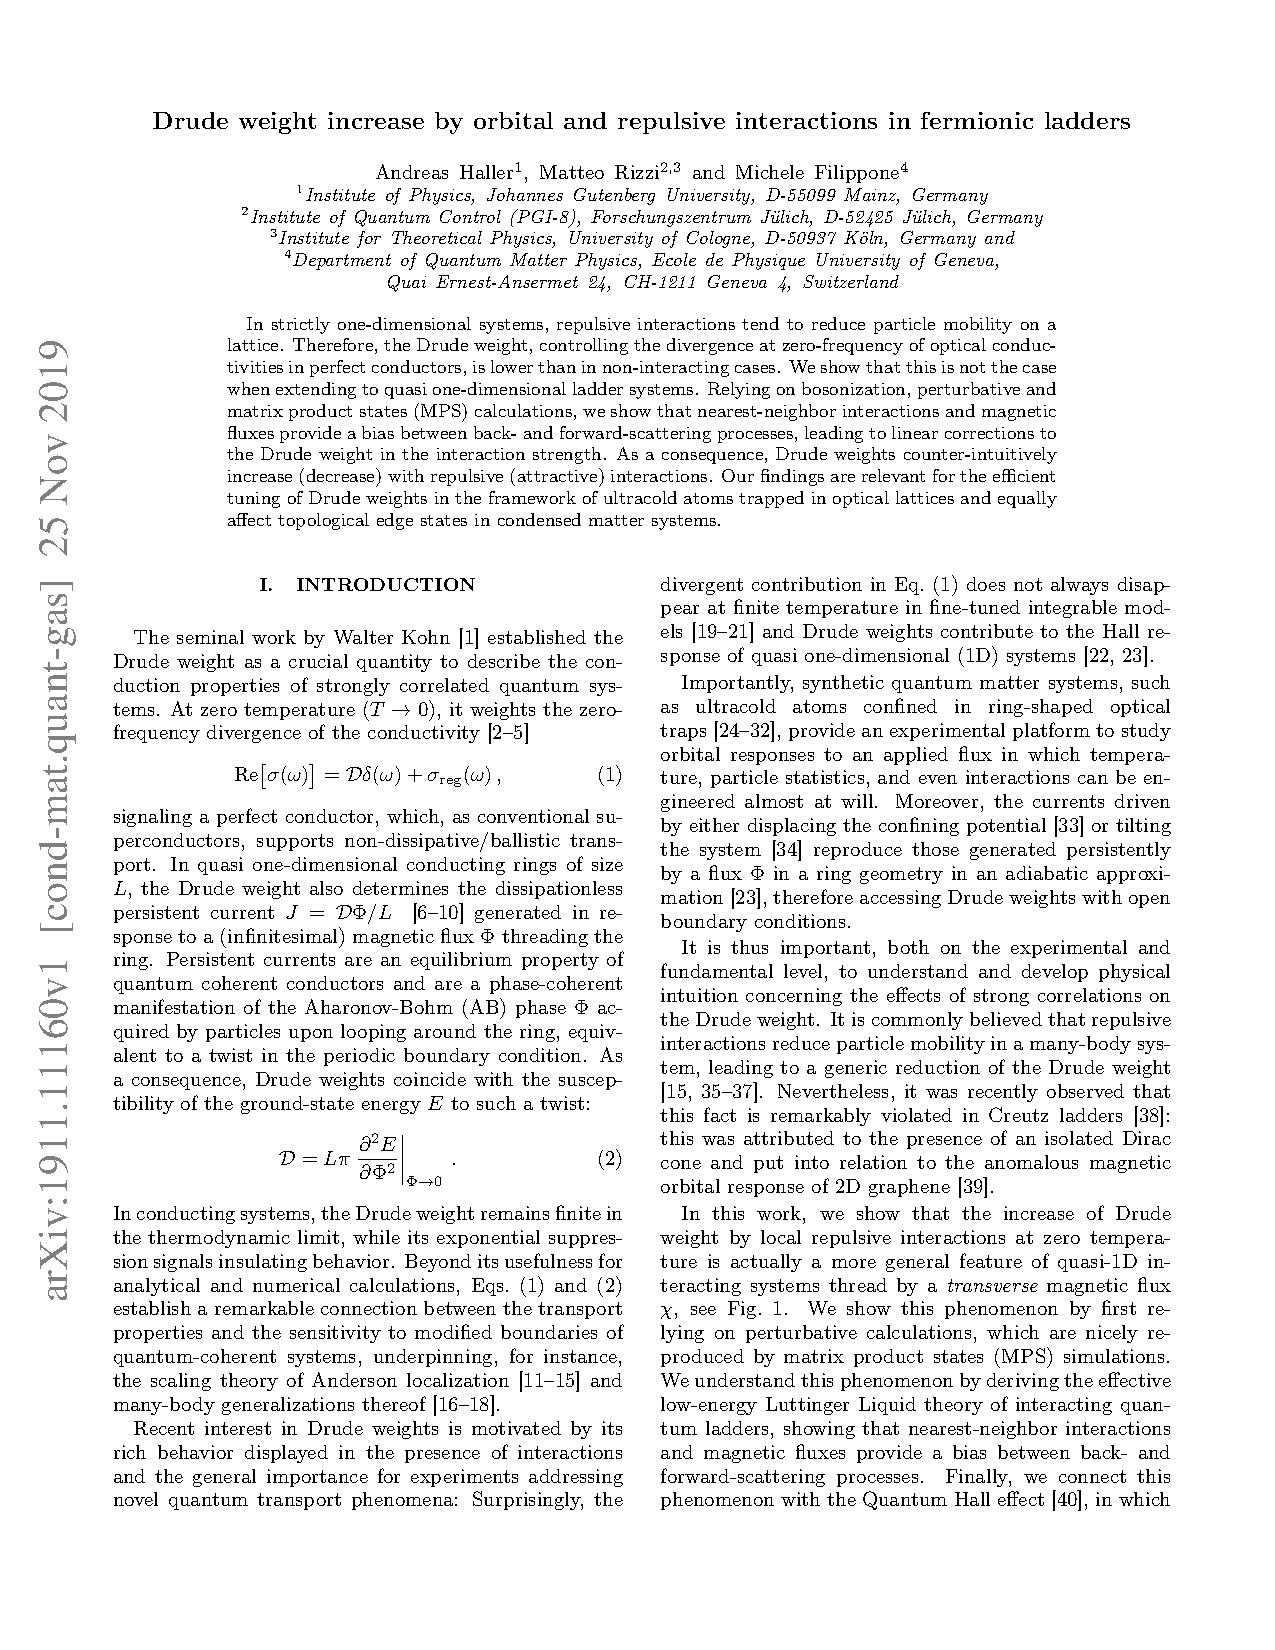
\includepdf[pages={1-},
addtotoc={
    1,chapter,1,Drude weight increase by orbital and repulsive interactions in fermionic ladders,drude_increased1,
    %
    1,section,1,Introduction,drude_increased2,
    %
    2,section,1,Weak Drude weight renormalization in one dimension,drude_increased3,
    %
    3,section,1,Model,drude_increased4,
    %
    4,section,1,Perturbation theory,drude_increased5,
    %
    6,section,1,Bosonization and connection to Quantum Hall systems,drude_increased6,
    %
    7,section,1,Discussion and conclusion,drude_increased7
}
]{Library/drude_increased.pdf}

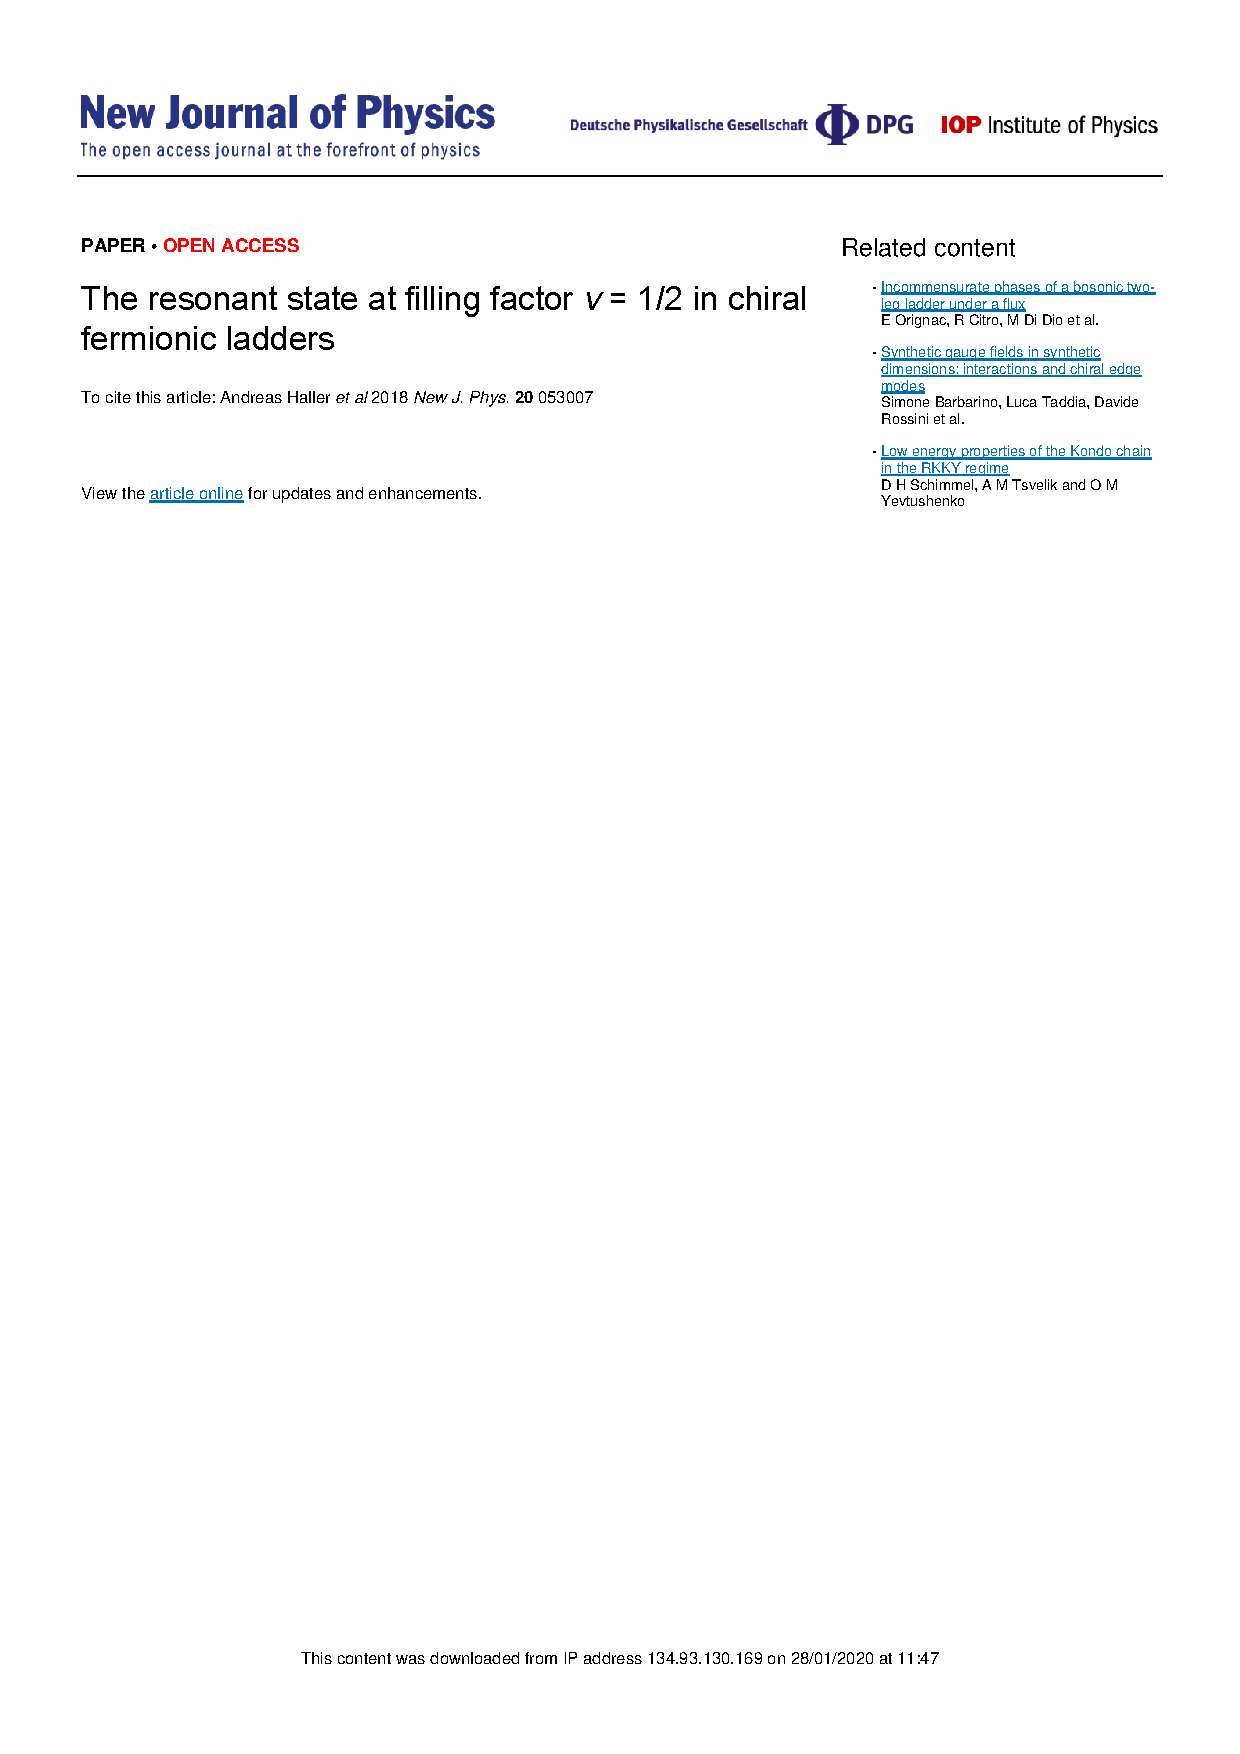
\includepdf[pages={2-},
addtotoc={
    2,chapter,1,The resonant state at filling factor \texorpdfstring{$\nu=1/2$}{nu=1/2} in chiral fermionic ladders,one_half1,
    %
    2,section,1,Introduction,one_half2,
    %
    3,section,1,The model,one_half3,
    %
    4,section,1,RG analysis,one_half4,
    %
    5,section,1,The entanglement properties,one_half5,
    %
    6,section,1,The correlations,one_half6,
    %
    7,section,1,Conclusions,one_half7
}
]{Library/pretopological_states_fermions.pdf}

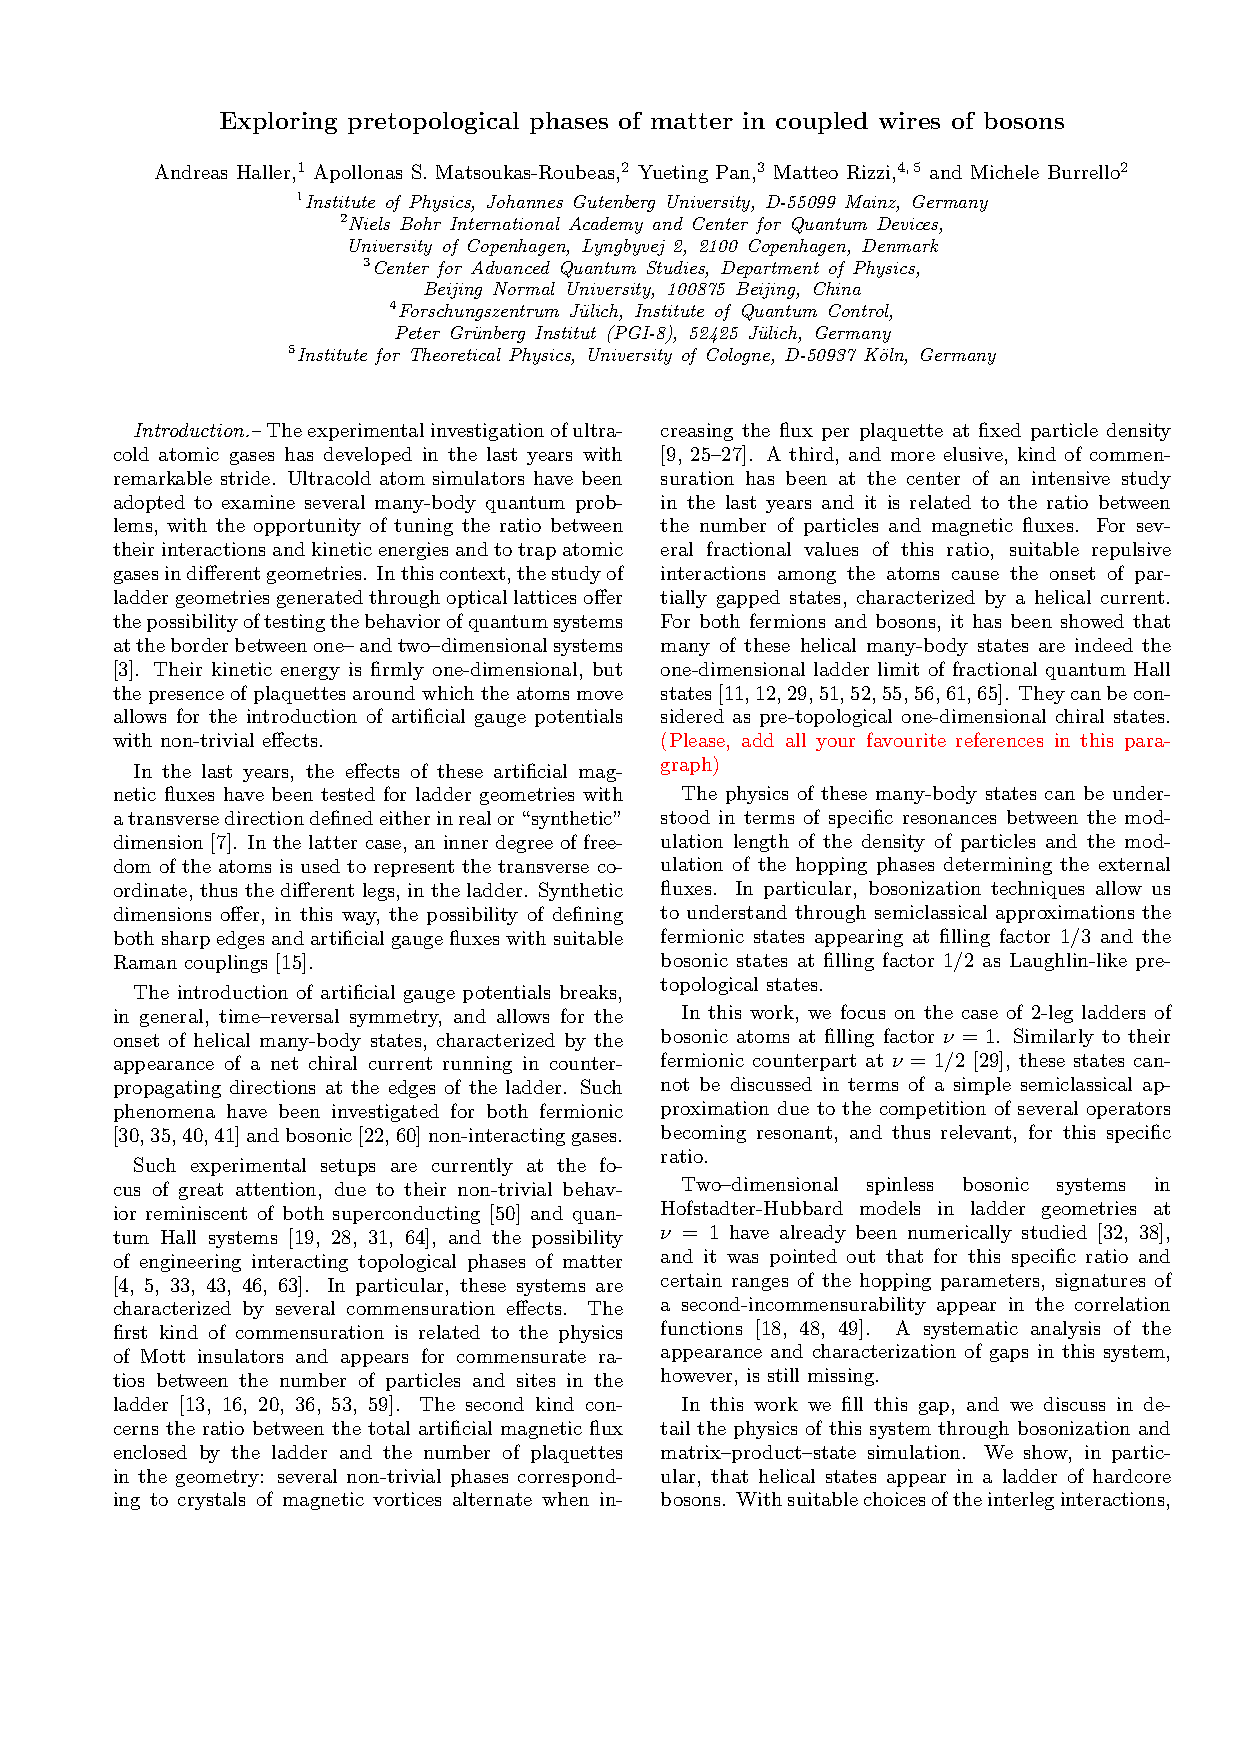
\includepdf[pages={1-},
addtotoc={
    1,chapter,1,Exploring helical phases of matter in bosonic ladders,integer1,
    %
    2,section,1,The model,integer2,
    %
    2,subsection,1,The single-particle physics,integer3,
    %
    3,subsection,1,Introducing the interactions,integer4,
    %
    3,section,1,Effective low-energy description of the model,integer5,
    %
    4,section,1,Renormalization group analysis,integer6,
    %
    7,section,1,Numerical results,integer7,
    %
    7,subsection,1,Chiral current,integer8,
    %
    9,subsection,1,Fluctuations and estimate of the Luttinger parameters,integer9,
    %
    10,subsection,1,Correlations,integer10,
    %
    11,subsection,1,Dynamics and velocities,integer11,
    %
    12,section,1,Conclusions and perspectives,integer12
}
]{Library/pretopological_states_bosons.pdf}

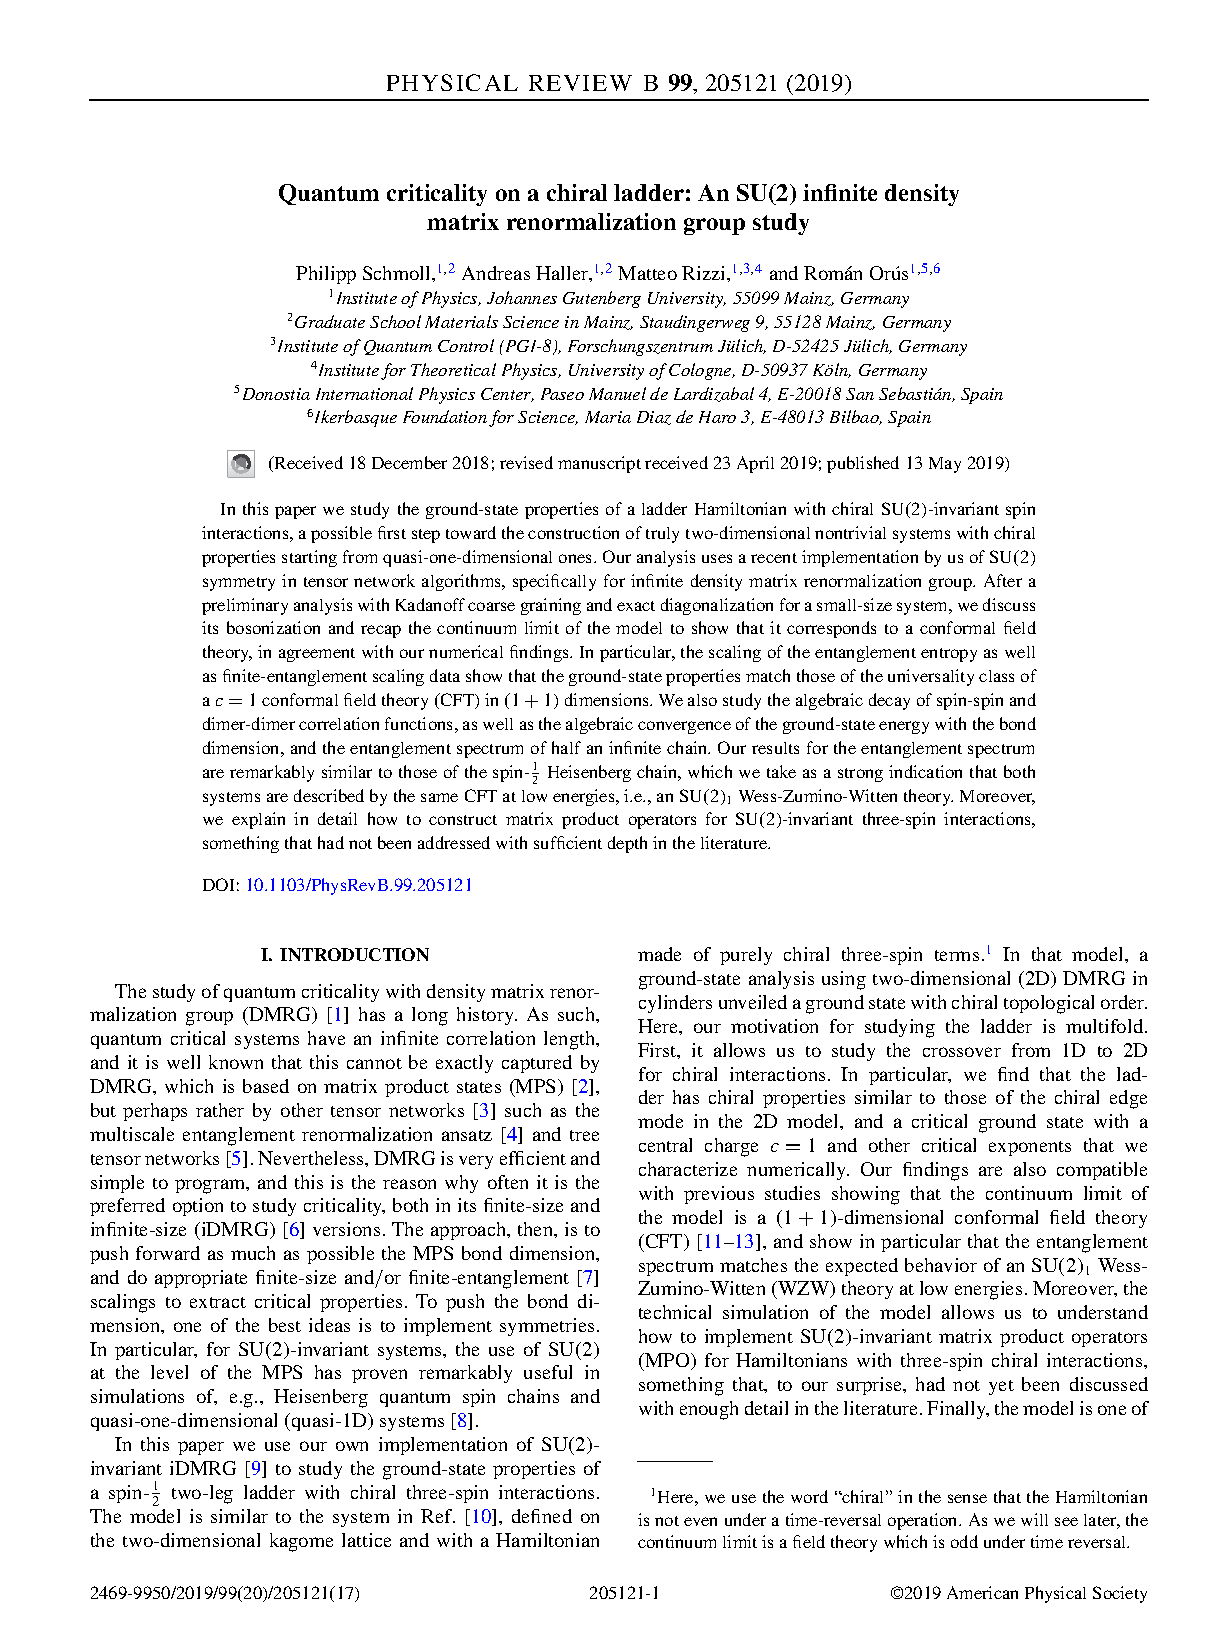
\includepdf[pages={1-},
addtotoc={
    1,chapter,1,Quantum criticality on a chiral ladder: An SU$(2)$ infinite density matrix renormalization group study,chiral1,
    %
    1,section,1,Introduction,chiral2,
    %
    2,section,1,Chiral ladder,chiral3,
    %
    2,subsection,1,Model,chiral4,
    %
    3,subsection,1,First intuition with Kadanoff coarse graining,chiral5,
    %
    3,subsection,1,Exact diagonalization of small systems,chiral6,
    %
    4,subsection,1,Bosonization,chiral7,
    %
    6,section,1,Methods,chiral8,
    %
    7,section,1,Results,chiral9,
    %
    7,subsection,1,Energy convergence,chiral10,
    %
    7,subsection,1,Entanglement,chiral11,
    %
    8,subsection,1,Correlation functions,chiral12,
    %
    9,subsection,1,Entanglement spectrum,chiral13,
    %
    9,section,1,Conclusions,chiral14
}
]{Library/spin_chain.pdf}

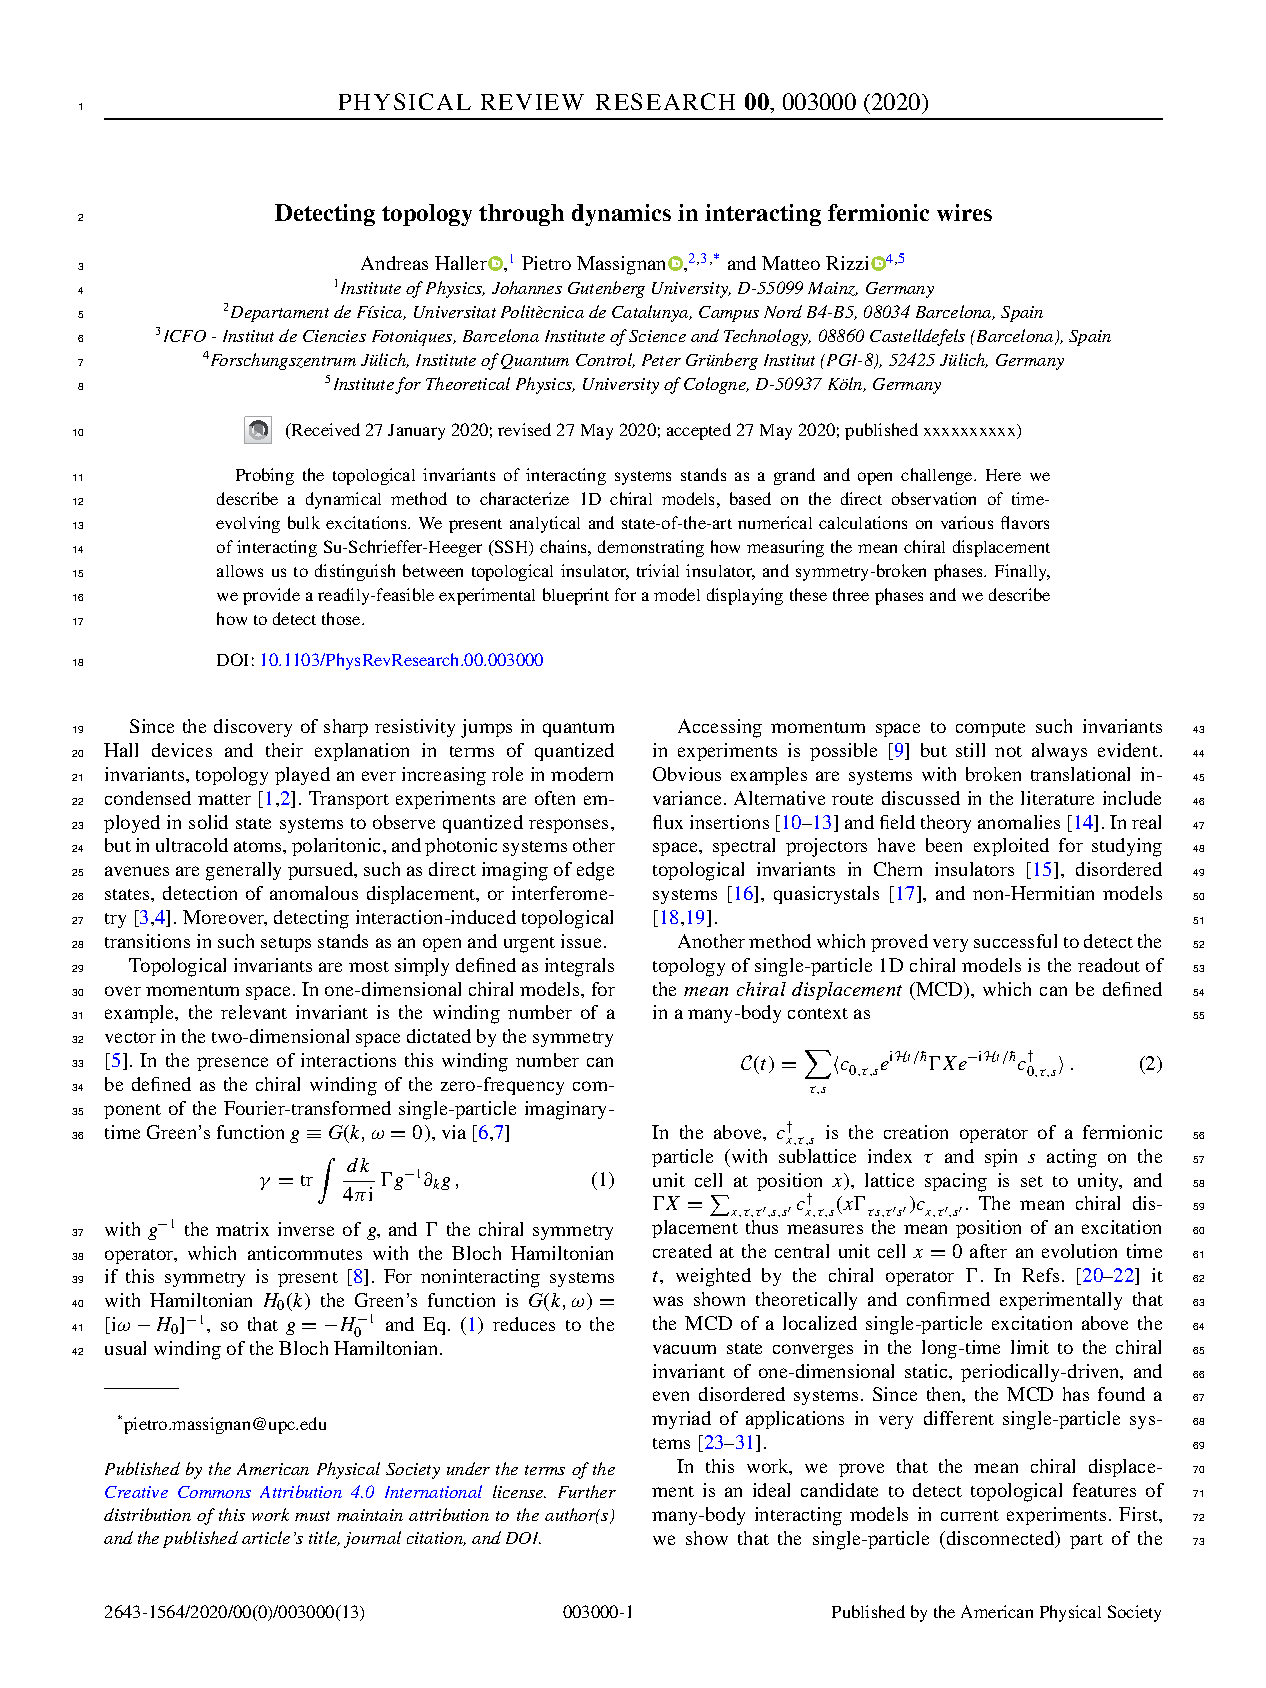
\includepdf[pages={1-},
addtotoc={
    1,chapter,1,Detecting topology through dynamics in interacting fermionic wires,mcd1,
    %
    2,section,1,Mean chiral displacement as a topological marker,mcd2,
    %
    2,section,1,Model: Interacting SSH chains,mcd3,
    %
    3,section,1,The noninteracting case,mcd4,
    %
    3,section,1,The short-ranged case,mcd5,
    %
    4,section,1,Effective interacting spin model,mcd6,
    %
    4,section,1,The long-ranged case,mcd7,
    %
    4,section,1,Experimental blueprint for $\MH_{\rm lr}$,mcd8,
    %
    4,section,1,Conclusions,mcd9
}
]{Library/mcd.pdf}
